\section{Informationstheoretische Vorbetrachtungen}
\subsection{Translatorische Orientierungssysteme}
\subsubsection{Himmelsrichtungen}
Ein dreidimensionaler Vektorraum habe die drei orthogonalen Basisvektoren $x$, $y$ und $z$. Mithilfe von Elementen des Vektorraumes soll die Position eines Flugobjekts repräsentiert werden.
Dabei können aussagekräftige Achsenbezeichner der Anschaulichkeit erheblich zutragen. Eine generische Bezeichnung mit $x$, $y$ und $z$ mag für sich genommen anschaulich sein, kann aber beispielsweise zu Kompatibilitätsproblemen bei der Systemintegration führen. Bei einem Flugobjekt, welches die Erdatmosphäre nicht verlässt, bietet sich an Himmelsrichtungen, also Nord oder Süd und Ost oder West zu verwenden ergänzt durch Bezeichner wie oben oder unten für den dritten Freiheitsgrad. Die Begriffe oben oder unten lassen keinen Zweifel an der Orientierung des Koordinatensystems beispielsweise in Bezug auf den Gravitationsvektor wohingegen eine Bezeichnung mit z uneindeutig ist. Insgesamt reduziert sich die Fehlerwahrscheinlichkeit.\\
Für diese Arbeit wurde das Basissystem Nord-Ost-Unten (NOU eng. NED) gewählt \ref{link:LocalTangent}.



\subsection{Rotatorische Orientierungssysteme}

\subsubsection{Einführung}
Für die Drehlagen- oder Rotationsgeschwindigkeitsmodellierung eines Objekts im dreidimensionalen Raum sind Fragen das statische und dynamische Verhalten betreffend signifikant.
Welche Repräsentationen eignen sich die Drehlage eines Objekts eindeutig zu beschreiben und wie lässt sich zwischen ihnen wechseln? Und welche Operatoren eignen sich den Übergang von einer Drehlage zur anderen zu beschreiben innerhalb eines Repräsentationssystem und zwischen Repräsentationssystemen?\\
Euler-, Kardanwinkel und Quaternionen sind Teil der Antwort \ref{link:Eulerwinkel}.

\subsubsection{Eulerwinkel}
Eulerwinkel bilden ein Winkeltripel welches die Drehlage eines Objekts im dreidimensionalen Raum beschreibt und sich auch zur Rotationsmodellierung eignet.\\
Tatsächlich ist es nicht zwingend notwendig drei Winkeländerungen zu kennen um eine beliebige Rotation im dreidimensionalen Raum durchzuführen. Solange man die Rotationsachse kennt, ist eine Winkeländerung um diese eine Achse ausreichend. Quaternionen, eine andere Form der Drehlage-Repräsentation, arbeiten stärker nach diesem Prinzip. In Eulerwinkelnotation wird eine Rotation $D$ durch drei Teilrotationen, beispielsweise $D_x$, $D_{y'}$ und $D_{x''}$, dargestellt welche sequenziell um drei lokale Teilrotationsachsen, hier $x$, $y$ und $z$, ausgeführt werden wobei die dritte Teilrotationsachse gleich der ersten \ref{link:Eulerwinkel}. Die Teilrotationsnummer ist gekennzeichnet durch die Anzahl der Apostrophe welche bei null starten.
Bei einer intrinsischen Rotation wird bei der zweiten und dritten Rotation um die aktuelle Achse des Objekts rotiert. Bei einer extrinsischen Rotation wird um ein fixes kartesisches Koordinatensystem gedreht \ref{link:Eulerwinkel}.
Sechs Permutationen von Eulerwinkelkonventionen existieren.
\begin{align}
	D_z-D_{x'}-D_{z''}\\
	D_z-D_{y'}-D_{z''}\\
	D_y-D_{z'}-D_{y''}\\
	D_y-D_{x'}-D_{y''}\\
	D_x-D_{y'}-D_{x''}\\
	D_x-D_{z'}-D_{x''}
\end{align}
Unterscheidet man extrinsische und intrinsische Winkelvariationen verdoppelt sich die Zahl.
\begin{center}
	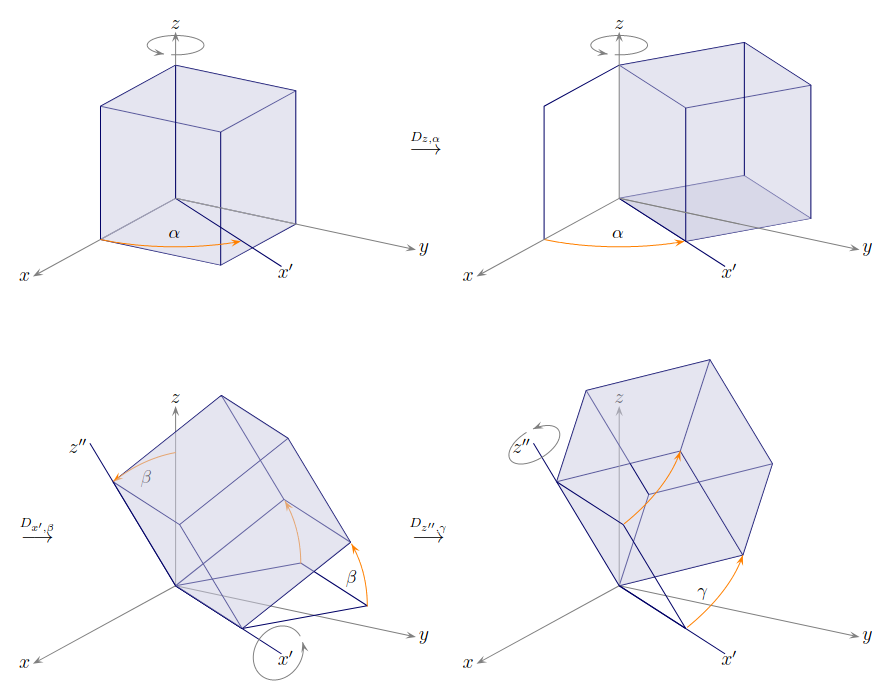
\includegraphics[scale=0.5]{../Bilder/0026 Eulerwinkel.png}{\\Intrinsische Rotationsmodellierung in Eulerwinkel bei z-x'-z'' Konvention \ref{bild:1}}
\end{center}
Ist die Drehlage eines Objekts durch Eulerwinkel definiert können Drehmatrizen herangezogen werden als Operatoren welche Drehlageänderungen beschreiben. Das Drehmatrizentripel welches mit Eulerwinkeln funktionieren hat 3x3 Matrizen als Elemente \ref{link:Eulerwinkel}. Die Rotationsmatrizen können achsenspezifisch wie folgt definiert werden
\begin{align}
	D_{x,\varphi} &= \begin{pmatrix}
		1 & 0 & 0\\
		0 & \cos{\varphi} & -\sin{\varphi}\\
		0 & \sin{\varphi} & \cos{\varphi}
	\end{pmatrix}\\
	D_{y,\varphi} &= \begin{pmatrix}
		\cos{\varphi} & 0 & \sin{\varphi}\\
		0 & 1 & 0\\
		-\sin{\varphi} & 0 & \cos{\varphi} 
	\end{pmatrix}\\
	D_{z,\varphi} &= \begin{pmatrix}
		\cos{\varphi} & -\sin{\varphi} & 0\\
		\sin{\varphi} & \cos{\varphi} & 0\\
		0 & 0 & 1
	\end{pmatrix}.
\end{align}
Rotationsmatrizen lassen sich zu einer Eulerrotation $D_{Euler}$ verketten
\begin{align}
	D_{Euler} &= D_{z, \alpha}\circ D_{x', \beta}\circ D_{z'', \gamma}. 
\end{align}
Mit der Matrizenmultiplikation als Operator berechnet sich $D_{Euler}$ zu folgender 3x3 Rotationsmatrizen
\begin{align}
	D_{Euler} &= \begin{pmatrix}
		\cos{\alpha}\cos{\gamma} - \sin{\alpha}\cos{\beta}\sin{\gamma} & -\cos{\alpha}\sin{\gamma} - \sin{\alpha}\cos{\beta}\cos{\gamma} & \sin{\alpha}\sin{\beta}\\
		\sin{\alpha}\cos{\gamma} + \cos{\alpha}\cos{\beta}\sin{\gamma} & -\sin{\alpha}\sin{\gamma} + \cos{\alpha}\cos{\beta}\cos{\gamma} & -\cos{\alpha}\sin{\beta}\\
		\sin{\beta}\sin{\gamma} & \sin{\beta}\cos{\gamma} & \cos{\beta}
	\end{pmatrix}.
\end{align}
Die Determinante und die Eigenwerte von Rotationsmatrizen sind +1. Wird eine Verkettung vieler Rotationsmatrizen numerische berechnet, kommt es aufgrund von Rundungsfehler zu einem abdriften der Eigenwerte. Um dem entgegenzuwirken werden die Drehlage-Vektoren in der Praxis periodisch normiert.

\subsubsection{Kardanwinkel}
Kardanwinkel welche auch als Tait-Bryan-Winkel genannt werden, gehören zur Klasse der Eulerwinkel sind aber keine Eulerwinkel im klassischen Sinne \ref{link:Eulerwinkel}. Im Gegensatz zu den klassischen Eulerwinkeln wird um jede Achse gedreht und nicht bei der dritten Drehung nochmal um die erste Achse.
\begin{center}
	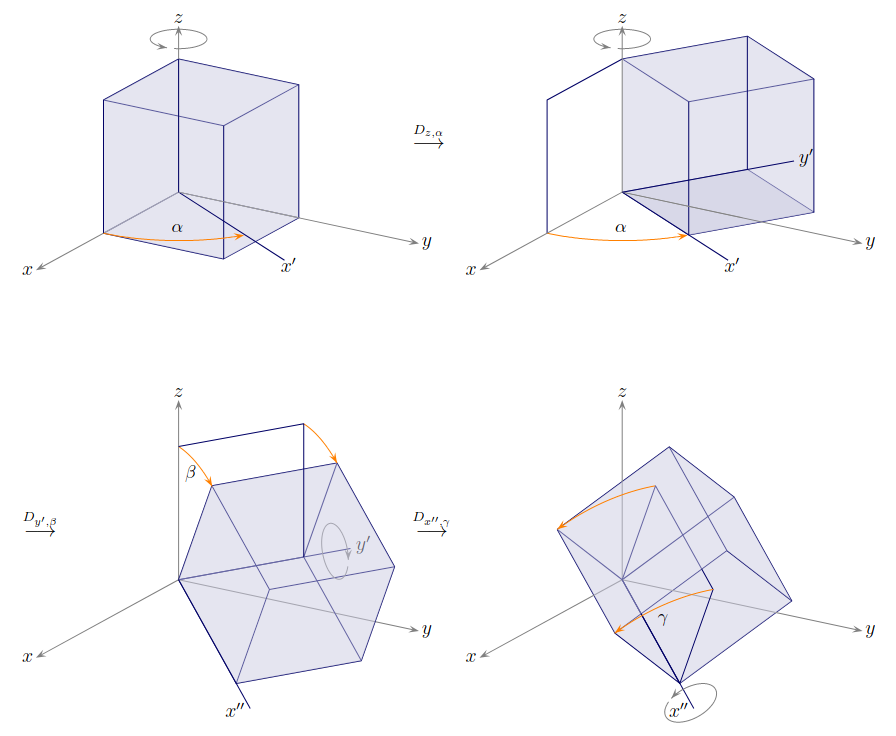
\includegraphics[scale=0.5]{../Bilder/0028 Kardanwinkel.png}{\\Intrinsische Rotationsmodellierung in Kardanwinkeln bei z-y-x Konvention \ref{bild:1}}
\end{center}
Es existieren auch Sechs Permutationen von Kardanwinkeln. 
\begin{align}
	D_x-D_{y'}-D_{z''}\\
	D_y-D_{x'}-D_{z''}\\
	D_x-D_{z'}-D_{y''}\\
	D_z-D_{x'}-D_{y''}\\
	D_z-D_{y'}-D_{x''}\\
	D_y-D_{z'}-D_{x''}
\end{align}
Die Drehlagerepräsentation des Quadcopters erfolgt in der Konvention $D_z-D_{y'}-D_{x''}$ also mit Kardanwinkeln, sofern nicht Quaternion zur Drehlagerepräsentation verwendet wurden.

\subsubsection{Flugsystemlage}
Flugzeuge, Helikopter, Quadcopter und Raketen sind Objekte welche beliebt im dreidimensionalen Raum orientiert sein können. Bei den genannten Objekten sind bestimmte Drehlagen zu gewissen Zeiten unerwünscht. Will man die Objekte in eine Solldrehlage bringen muss man ihre Drehlage quantifizieren. Dazu eignen sich Kardanwinkel. Besser geeignet sind Kardanwinkel mit modellspezifischer Achsenbezeichnung. Fachleute sprechen aus diesem Grund von Rollwinkel $\phi$, Nickwinkel $\theta$ und Gierwinkel $\psi$ \ref{link:SimCon}.
Die Fluglagenwinkel können zu einem Vektor
\begin{align}
	\varphi &= \begin{pmatrix}
		\phi\\
		\theta\\
		\psi
	\end{pmatrix}
	\Leftrightarrow 
	\begin{pmatrix}
		D_{x''}\\
		D_{y'}\\
		D_{z}
	\end{pmatrix}.
\end{align}
zusammengefasst werden. Zu erkennen ist zudem die gewählte Äquivalentbeziehung zwischen Kardanwinkeln und Fluglagenwinkeln.
\begin{center}
	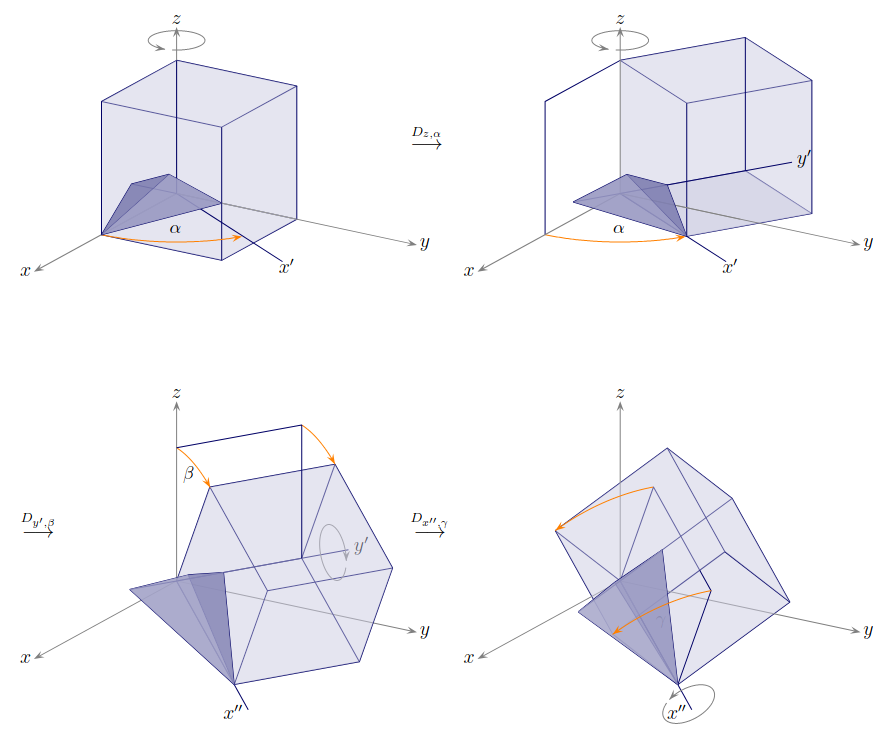
\includegraphics[scale=0.5]{../Bilder/0029 Roll-Pitch-Yaw.png}{\\Zunächst wird gegiert, dann genickt und dann gerollt. Die Winkelvorzeichen wurden für alle Implementierungen übernommen. \ref{bild:1}}
\end{center}

\subsubsection{Gimbel Lock}
Eulerwinkel punkten in Sachen anschaulich haben aber ein signifikantes strukturelles Problem.
Wird beispielsweise zunächst mit einem beliebigen Winkel $\alpha$ um die z-Achse gedreht, dann mit dem Winkel $\frac{\pi}{2}$ um die $y'$-Achse entspricht die dritte Rotationsachse der Ersten \ref{link:Eulerwinkel}. Immer wenn das der Fall ist, geht ein Freiheitsgrad verloren und der Zustand Gimbel-Lock tritt ein. Die Bezeichnung ist entstanden, weil kardanischen Lagerungen (eng. Gimbel) welche bei Messinstrumenten zum Einsatz kommen in den unerwünschten Zustand gebracht werden können.
\begin{center}
	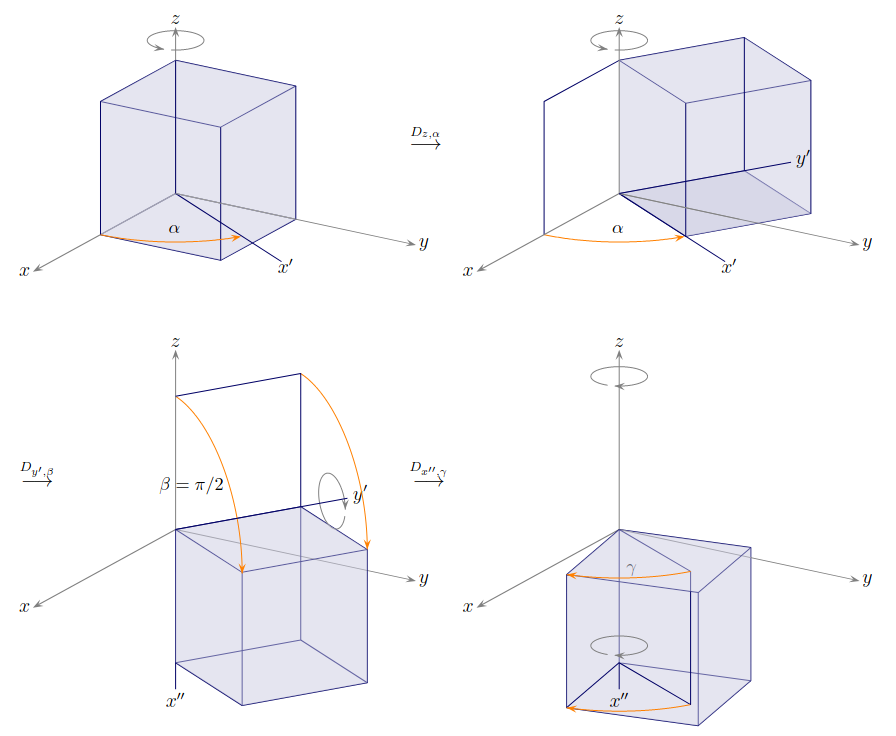
\includegraphics[scale=0.5]{../Bilder/0027 Gimbel Lock.png}{\\Gimbel Lock auf der z-Achse nachdem zweimal um die z-Achse gedreht wird. \ref{bild:1}}
\end{center}


\subsubsection{Quaternionen}
Eulerwinkel sind anschaulich aber nicht besonders handlich für die mathematische Modellierung von Drehlagen und Rotationsprozessen. Grund dafür ist unter anderem Gimbel Lock.\\
Quaternionen sind vierdimensionale Zahlen mit speziellen Eigenschaften die insbesondere aufgrund von ihren, die Zustandseindeutigkeit und Laufzeit betreffenden Vorteilen, im Bereich der Drehlagen und Rotationsprozesse eingesetzt werden. Eine Quaternion
\begin{align}
	q &= q_w + iq_x + jq_y + kq_z,\ q_w, q_x, q_y, q_z \in R
\end{align}
wird in kartesischer Form notiert mit drei imaginären Einheiten $i$, $j$ und $k$ welche allesamt Lösungen für negative Einheitswurzeln sind
\begin{align}
	i &= j = k = \sqrt{-1}.
\end{align}
Die Norm einer Quaternion $|q|$ entspricht dem euklidischen Abstand berechnet auf allen Elementen
\begin{align*}
	|q| &= \left (q_w^2 + q_x^2 + q_y ^ 2 + q_z ^ 2\right )^{\frac{1}{2}}.
\end{align*}
Oft ist es notwendig eine Quaternion zu normieren da die Rotationsmodellierung nur mit Einheitsquaternionen funktioniert.
\begin{align}
	\frac{q}{|q|} &= \frac{q_w}{|q|} + i\frac{q_x}{|q|} + j\frac{q_y}{|q|} + k\frac{q_z}{|q|}
\end{align}
Zu jeder Quaternion existiert mit
\begin{align}
	q^{-1} &= \frac{1}{|q|}(q_w - iq_x - jq_y - kq_z)
\end{align}
eine Inverse für die gilt
\begin{align}
	qq^{-1} &= q^{-1}q = 1.
\end{align}
Geht man von einer Rotation in Form von einem Winkel
\begin{align}
	\theta &\in [0, 2\pi]
\end{align}
und einem Eulervektor
\begin{align}
	v &= \begin{pmatrix}
		v_x\\
		v_y\\
		v_z
	\end{pmatrix}
	\in R^3
\end{align} 
als einen Vektor mit Elementen eines dreidimensionalen Vektorraumes aus und will diesen als Quaternion ausdrücken kann dies über trigonometrische Funktionen passieren
\begin{align}
	\begin{pmatrix}
		q_w\\
		q_x\\
		q_y\\
		q_z
	\end{pmatrix}
	&= \begin{pmatrix}
		\cos\left (\frac{\theta}{2}\right )\\
		v_x \sin \left (\frac{\theta}{2}\right )\\
		v_y \sin \left (\frac{\theta}{2}\right )\\
		v_z \sin \left (\frac{\theta}{2}\right )
	\end{pmatrix}.
\end{align}
Soll ein Vektor oder Punkt $p = (p_x, p_y, p_z) \in R^3$ im dreidimensionalen Raum rotiert werden transformiert man zunächst den Vektor in eine Quaternion, indem der Realteil zu null gesetzt wird und die drei Imaginärteile aufsteigend mit den Elementen des Vektors gleichsetzt werden
\begin{align}
	q_p &= \begin{pmatrix}
		0\\
		p_x\\
		p_y\\
		p_z
	\end{pmatrix}.
\end{align}
Die Rotation wird nun berechnet, indem zunächst die Rotationsquaternion auf $q_p$ multipliziert wird und dann die Inverse der Rotationsquaternion multipliziert wird
\begin{align}
	q_p' &= qq_pq^{-1}.
\end{align}
Kardanwinkel lassen sich zu einer Quaternion umrechnen
\begin{align*}
	\begin{pmatrix}
		q_w\\
		q_x\\
		q_y\\
		q_z
	\end{pmatrix}
	&=
	\frac{1}{|q|}
	\begin{pmatrix}
		\cos(0.5\psi)\cos(0.5\theta)\cos(0.5\phi) + \sin(0.5\psi)\sin(0.5\theta)\sin(0.5\phi)\\
		\cos(0.5\psi)\cos(0.5\theta)\sin(0.5\phi) - \sin(0.5\psi)\sin(0.5\theta)\cos(0.5\phi)\\
		\cos(0.5\psi)\sin(0.5\theta)\cos(0.5\phi) + \sin(0.5\psi)\cos(0.5\theta)\cos(0.5\phi)\\
		\sin(0.5\psi)\cos(0.5\theta)\cos(0.5\phi) - \cos(0.5\psi)\sin(0.5\theta)\cos(0.5\phi)
	\end{pmatrix}
\end{align*}
und die Umkehrabbildung ist, ebenfalls nach \ref{link:Quaternion}, folgende
\begin{align}
	\begin{pmatrix}
		\psi\\
		\theta\\
		\phi
	\end{pmatrix}
	&= 
	\begin{pmatrix}
		\text{arctan}\left (\frac{2(q_xq_y + q_0q_z)}{q_w ^ 2 + q_x ^ 2 - q_y ^ 2 - q_z ^ 2}\right )\\
		\text{arcsin}\left (-2(q_yq_z + q_wq_x)\right )\\
		\text{arctan}\left (\frac{2(q_yq_z+q_wq_x)}{q_w ^ 2 - q_x ^ 2 - q_y ^ 2 + q_z ^ 2}\right )
	\end{pmatrix}.
\end{align}
